\section{ねじりと曲げを受ける長方形の棒}
このケースでは、複合荷重(ねじりと曲げ)を受ける長方形断面の棒を解析します。その寸法は:
\begin{itemize}
\item 断面:200$\times$300mmの長方形
\item 長さ:1400mm
\end{itemize}
\begin{enumerate}
\item
  {[}mm, ton, s, °C{]}単位の新規ファイルを作成し、ステップ形式のジオメトリをPrePoMaxにインポートします。
  次に、パーツをメッシュ分割します。
  ここでは、最大要素サイズとして30mmを選択し、その他の設定は変更しませんでした(図\ref{fig:04-01})。
	\begin{figure}[H]
	\centering
	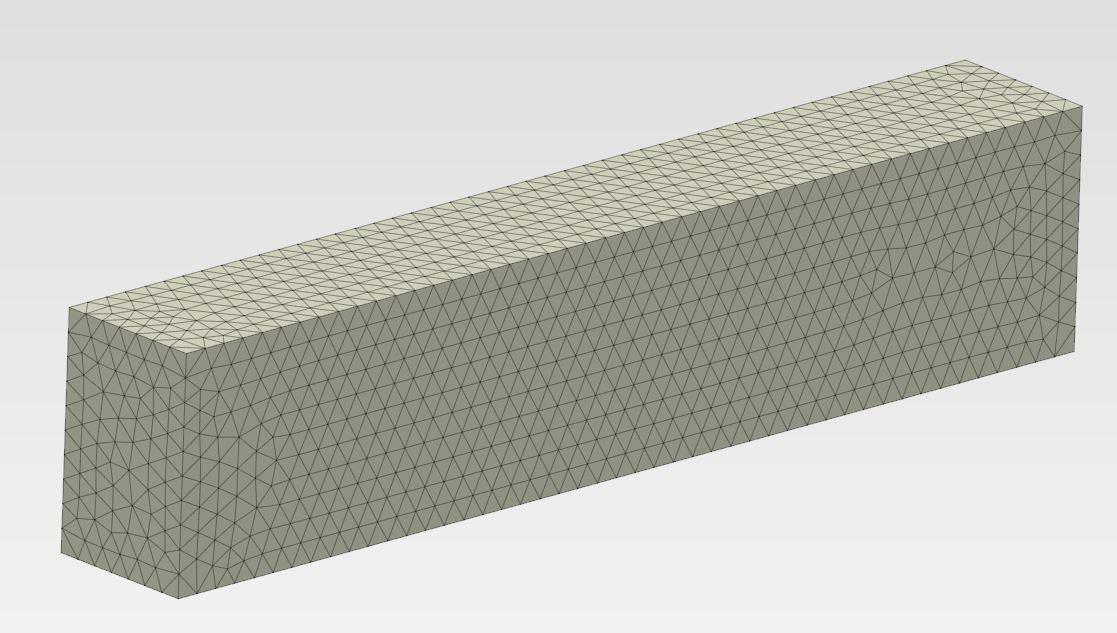
\includegraphics[width=125mm]{fig/04-01.png}
	\caption{長方形の棒 - メッシュ}
	\label{fig:04-01}
	\end{figure}
\vspace{-\baselineskip}
\item
  新しい材料を定義し、弾性挙動を加え、ヤング率を180000MPa、ポアソン比を0.25と指定します。
  先に作成した材料を参照して新しいソリッドセクションを作成し、そのセクションがこのパーツに割り当てられるように棒を選択します。
\item
  座標(500, 0, 1400)に基準点を作成します。
  この基準点を使って剛体拘束を作成し、棒の表面に割り当てます。
\item
  デフォルトの設定で静的解析ステップを定義します。
  固定境界条件を基準点のある方と反対側の棒の端に割り当てます。
  もう一方の棒には集中荷重を設定します。棒の軸に垂直な方向に-8000Nの値を指定します(図\ref{fig:04-02})。
	\begin{figure}[H]
	\centering
	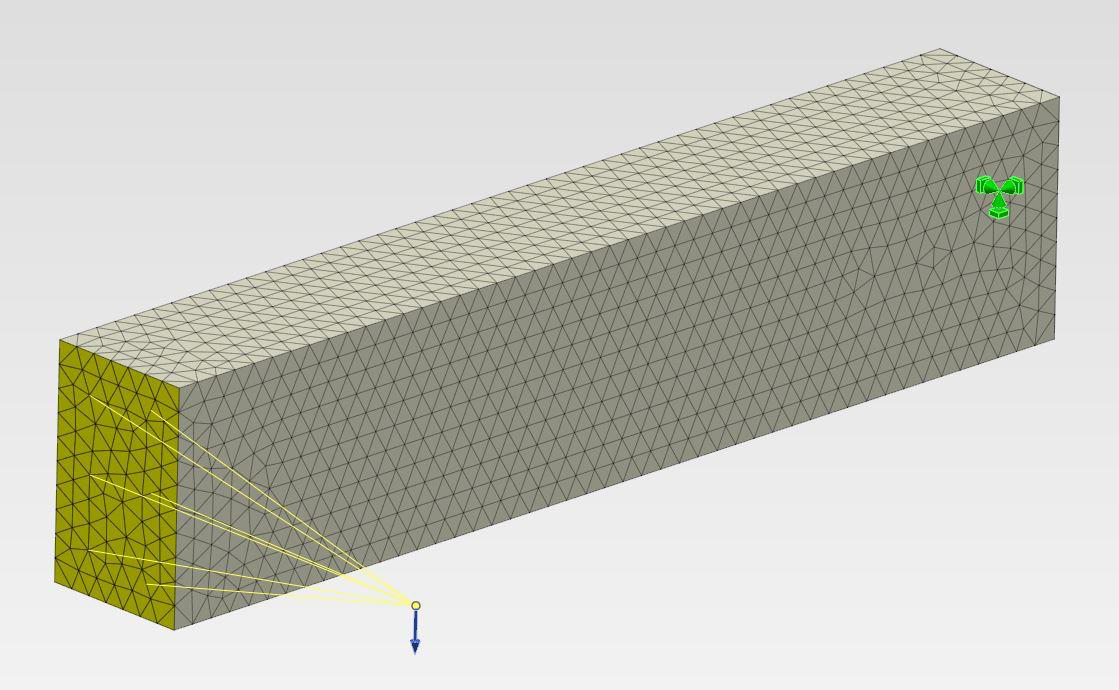
\includegraphics[width=135mm]{fig/04-02.png}
	\caption{長方形の棒 - 境界条件と荷重}
	\label{fig:04-02}
	\end{figure}
\vspace{-\baselineskip}
\item
  解析を実行し、結果を確認します。
  変形のスケール係数を1000に設定し、非変形モデルを描画するオプションを有効にします(図\ref{fig:04-03})。
  リモート荷重によってバーが曲げられたり、ねじられたりしているのがわかります。
  解析結果は4.69MPa程度です。
  シミュレーション結果は応力集中とメッシュ感度の影響を受けますが、この場合、最大応力があるコーナーのすぐ隣のノードで読み取られた値は4.77MPaです。
\vspace{-.5\baselineskip}
	\begin{figure}[H]
	\centering
	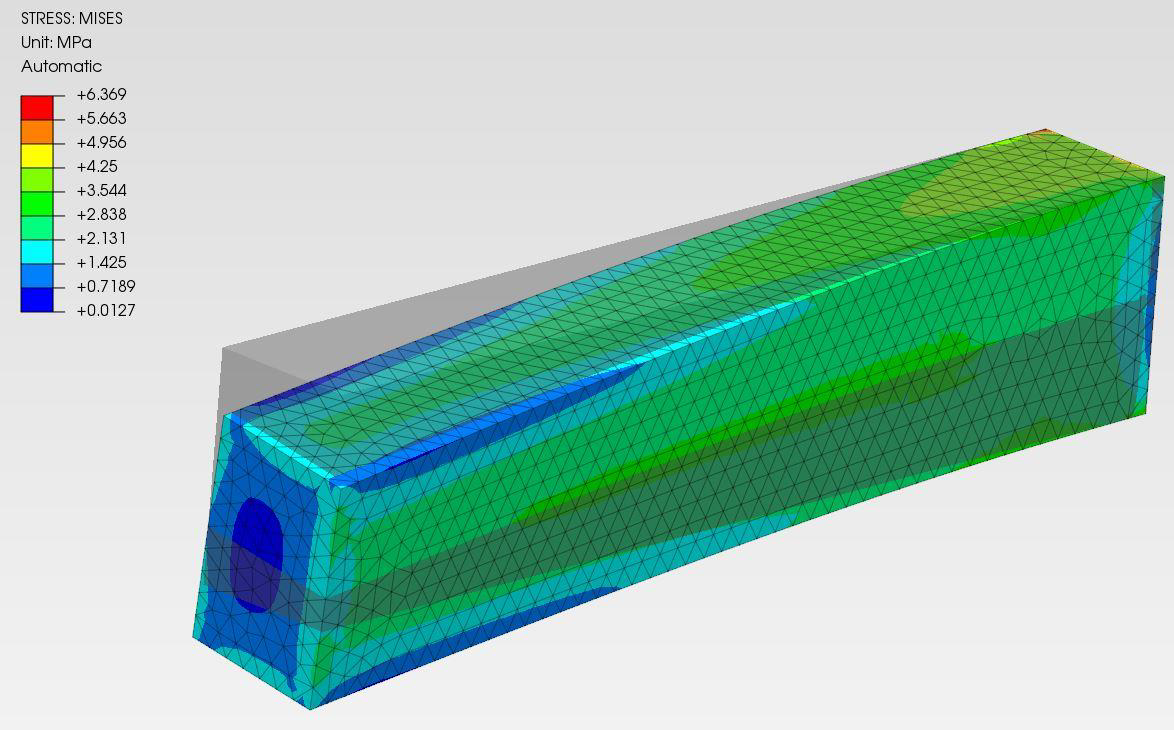
\includegraphics[width=135mm]{fig/04-03.png}
	\caption{長方形の棒 - フォンミーゼス応力}
	\label{fig:04-03}
	\end{figure}
\end{enumerate}